%%%%%%%%%%%%%%%%%%%%%%%%%%%%%%%%%%%%%%%%%
% Masters/Doctoral Thesis 
% LaTeX Template
% Version 2.4 (22/11/16)
%
% This template has been downloaded from:
% http://www.LaTeXTemplates.com
%
% Version 2.x major modifications by:
% Vel (vel@latextemplates.com)
%
% This template is based on a template by:
% Steve Gunn (http://users.ecs.soton.ac.uk/srg/softwaretools/document/templates/)
% Sunil Patel (http://www.sunilpatel.co.uk/thesis-template/)
%
% Template license:
% CC BY-NC-SA 3.0 (http://creativecommons.org/licenses/by-nc-sa/3.0/)
%
%%%%%%%%%%%%%%%%%%%%%%%%%%%%%%%%%%%%%%%%%

%----------------------------------------------------------------------------------------
%	PACKAGES AND OTHER DOCUMENT CONFIGURATIONS
%----------------------------------------------------------------------------------------

\documentclass[
12pt, % The default document font size, options: 10pt, 11pt, 12pt
oneside, % Two side (alternating margins) for binding by default, uncomment to switch to one side
italian, % ngerman for German
onehalfspacing, % Single line spacing, alternatives: onehalfspacing or doublespacing
%draft, % Uncomment to enable draft mode (no pictures, no links, overfull hboxes indicated)
%nolistspacing, % If the document is onehalfspacing or doublespacing, uncomment this to set spacing in lists to single
%liststotoc, % Uncomment to add the list of figures/tables/etc to the table of contents
%toctotoc, % Uncomment to add the main table of contents to the table of contents
%parskip, % Uncomment to add space between paragraphs
%nohyperref, % Uncomment to not load the hyperref package
headsepline, % Uncomment to get a line under the header
chapterinoneline, % Uncomment to place the chapter title next to the number on one line
%consistentlayout, % Uncomment to change the layout of the declaration, abstract and acknowledgements pages to match the default layout
]{MastersDoctoralThesis} % The class file specifying the document structure

\usepackage[utf8]{inputenc} % Required for inputting international characters
\usepackage[T1]{fontenc} % Output font encoding for international characters
\let\latinencoding\relax
\usepackage{fontspec} % Better font handling

\usepackage[newfloat]{minted} % Code Highlighting
\usepackage{caption}
\usepackage{tcolorbox}
\usepackage{etoolbox}

\newenvironment{code}{\captionsetup{type=listing}}{}
\SetupFloatingEnvironment{listing}{name=Snippet}

\BeforeBeginEnvironment{minted}{\begin{tcolorbox}}%
\AfterEndEnvironment{minted}{\end{tcolorbox}}%


\setmainfont{Palatino Linotype}
\setmonofont[Scale=0.85]{Consolas}

\usepackage[backend=bibtex,style=numeric,natbib=true]{biblatex} % Use the bibtex backend with the authoryear citation style (which resembles APA)

\addbibresource{bibliography.bib} % The filename of the bibliography

\usepackage[autostyle=true]{csquotes} % Required to generate language-dependent quotes in the bibliography

\newcommand*\justify{%
    \fontdimen2\font=0.4em% interword space
    \fontdimen3\font=0.2em% interword stretch
    \fontdimen4\font=0.1em% interword shrink
    \fontdimen7\font=0.1em% extra space
    \hyphenchar\font=`\-% allowing hyphenation
}


%----------------------------------------------------------------------------------------
%	MARGIN SETTINGS
%----------------------------------------------------------------------------------------

\geometry{
	paper=a4paper, % Change to letterpaper for US letter
	inner=2.5cm, % Inner margin
	outer=3.8cm, % Outer margin
	bindingoffset=1cm, % Binding offset
	top=3.5cm, % Top margin
	bottom=3cm, % Bottom margin
	%showframe, % Uncomment to show how the type block is set on the page
}

%----------------------------------------------------------------------------------------
%	THESIS INFORMATION
%----------------------------------------------------------------------------------------

\thesistitle{Sviluppo di un Sistema di Previsione di Ritardi Aerei Basato su Big Data} % Your thesis title, this is used in the title and abstract, print it elsewhere with \ttitle
\supervisor{Dott. Luca \textsc{Oneto}} % Your supervisor's name, this is used in the title page, print it elsewhere with \supname
\examiner{} % Your examiner's name, this is not currently used anywhere in the template, print it elsewhere with \examname
\degree{Corso di Laurea Magistrale in Ingegneria Informatica} % Your degree name, this is used in the title page and abstract, print it elsewhere with \degreename
\author{Enrico \textsc{Ferro}} % Your name, this is used in the title page and abstract, print it elsewhere with \authorname
\addresses{} % Your address, this is not currently used anywhere in the template, print it elsewhere with \addressname

\subject{Data Analysis} % Your subject area, this is not currently used anywhere in the template, print it elsewhere with \subjectname
\keywords{} % Keywords for your thesis, this is not currently used anywhere in the template, print it elsewhere with \keywordnames
\university{{Università degli studi di Genova}} % Your university's name and URL, this is used in the title page and abstract, print it elsewhere with \univname
\department{\href{http://www.dibris.unige.it/}{DIBRIS - Department of Informatics, Bioengineering, Robotics and Systems Engineering}} % Your department's name and URL, this is used in the title page and abstract, print it elsewhere with \deptname
\group{\href{http://researchgroup.university.com}{Research Group Name}} % Your research group's name and URL, this is used in the title page, print it elsewhere with \groupname
\faculty{\href{http://www.informatica.ingegneria.unige.it/}{Ingegneria Informatica}} % Your faculty's name and URL, this is used in the title page and abstract, print it elsewhere with \facname

\AtBeginDocument{
\hypersetup{pdftitle=\ttitle} % Set the PDF's title to your title
\hypersetup{pdfauthor=\authorname} % Set the PDF's author to your name
\hypersetup{pdfkeywords=\keywordnames} % Set the PDF's keywords to your keywords
}

\begin{document}
\hypersetup{colorlinks, urlcolor=blue, linkcolor=blue}

\frontmatter % Use roman page numbering style (i, ii, iii, iv...) for the pre-content pages

\pagestyle{plain} % Default to the plain heading style until the thesis style is called for the body content

%----------------------------------------------------------------------------------------
%	TITLE PAGE
%----------------------------------------------------------------------------------------

\begin{titlepage}
%\linespread{1.5}
\thispagestyle{empty}
\begin{center}
	
\includegraphics[width=0.2\linewidth]{Figures/unige.eps}
\end{center}

\begin{center}
	\LARGE\sc
	\univname\\
	
	\vspace{0.5cm}
	\large
	\degreename\\
\end{center}

\begin{center}
	\small
	Tesi di Laurea per il conseguimento del titolo di\\
	Dottore Magistrale in Ingegneria Informatica\\
\end{center}

\vfill

\begin{center} 
	\LARGE
	{\bf \ttitle}\\
	\vspace{0.5cm}
	\large
	\authorname\\
	\vspace{0.5cm}
	\small
	Anno Accademico 2016/2017
\end{center}

\vfill

\begin{tabular}{lll}%
	{\em Relatore}:	& Luca Oneto\\
	{\em Relatore}:	& Davide Anguita\\
    {\em Correlatore}: & Alberto Galletto
\end{tabular} 

\hfill


\end{titlepage}


%----------------------------------------------------------------------------------------
%	QUOTATION PAGE
%----------------------------------------------------------------------------------------

%\vspace*{0.2\textheight}

%\noindent\enquote{\itshape Thanks to my solid academic training, today I can write hundreds of words on virtually any topic without possessing a shred of information, which is how I got a good job in journalism.}\bigbreak

%\hfill Dave Barry

%----------------------------------------------------------------------------------------
%	ABSTRACT PAGE
%----------------------------------------------------------------------------------------

\begin{abstract}
Nel corso degli ultimi anni si è sempre più affermata l'importanza di avere grandi quantità di dati a disposizione ed una maggiore consapevolezza delle potenzialità dei Big Data. Questa tesi è volta a mostrare i componenti e le fasi di sviluppo necessarie alla definizione di un sistema di analisi dati, in grado di ottenere modelli predittivi a partire dall'enorme mole di informazioni a disposizione. Diversi approcci sono disponibili allo stato dell'arte in tale ambito e lo studio si è concentrato, in particolare, sulle potenzialità e affidabilità di tecnologie che permettano l'elaborazione in tempo reale. Avvalendosi del framework Apache Spark per l'elaborazione distribuita su un'infrastruttura Big Data basata sulla suite Hadoop, è stato applicato il metodo delle Random Forest per la predizione dei ritardi aerei a partire dalle statistiche di volo fornite dal servizio di air monitoring FlightAware. All'infrastruttura sono stati aggiunti un sistema di notifiche mobile per la fruizione delle analitiche ottenute e un perimetro di sicurezza per proteggere l'intera struttura. I risultati avuti dal particolare caso osservato hanno dimostrato l'efficacia e accuratezza degli strumenti adottati.
\end{abstract}

\tableofcontents % Prints the main table of contents

%----------------------------------------------------------------------------------------
%	DEDICATION
%----------------------------------------------------------------------------------------

%\dedicatory{For/Dedicated to/To my\ldots} 

%----------------------------------------------------------------------------------------
%	THESIS CONTENT - CHAPTERS
%----------------------------------------------------------------------------------------

\mainmatter % Begin numeric (1,2,3...) page numbering

\pagestyle{thesis} % Return the page headers back to the "thesis" style

% Include the chapters of the thesis as separate files from the Chapters folder
% Uncomment the lines as you write the chapters

\chapter{Introduzione}

\section{I Big Data}
Con questo termine, sempre più diffuso nell'immaginario comune, si vuole indicare una grande mole di dati, strutturati e non, con il potenziale per ricavare ulteriori informazioni e indurre nuove riflessioni riguardo all'ambito considerato.\\
Sebbene la parola in sè sia stata coniata recentemente, l'ambiente che rappresentano ha origini molto più radicate e, con il tempo, si è diffusa la definizione descritta dalle tre \textbf{V}:

\begin{itemize}
	\item \textbf{Volume}: la quantità di dati manipolati deve essere enorme, non gestibile da un sistema tradizionale. Si parla di grandezze dell'ordine degli \textit{zettabytes}, ovvero $10^{21}$ bytes, che devono essere assunte dal sistema e memorizzate per l'analisi. Ogni dato può contenere risvolti rilevanti ed è fondamentale essere sicuri di non perdere nulla. 
	
	\item \textbf{Velocity}: i sistemi Big Data devono tenere il passo con i servizi che vengono loro richiesti. Applicazioni legate al mondo dell'IoT (Internet of Things) e alla sensorizzazione di alcune azioni quotidiane necessitano tempi di risposta veloci e ritmi di lavoro compassati.
	
	\item \textbf{Variety}: bisogna essere pronti a operare su dati eterogenei, in quanto la grande disponibilità di dati non implica un corrispondente aumento di dati strutturati. Dunque, oltre ai classici databases e tabelle, ci si trova a lavorare con immagini, audio o documenti di testo.
\end{itemize}
Con il tempo a queste si sono aggiunte due ulteriori \textbf{V}, più inerenti alla sfera produttiva:

\begin{itemize}
	\item \textbf{Veracity}: ovvero la misura di fiducia che abbiamo nei dati a disposizione. Data la varietà di sorgenti cui si attinge e la velocità con cui le informazioni possono variare nel tempo, non è raro che tali fattori intacchino l'integrità dell'analisi ed è, dunque, fondamentale considerare tale eventualità e tenerne conto, cercando di limitarla quanto più possibile.
	
	\item \textbf{Value}: il valore delle informazioni che tali dati portano con sè. Un ambiente Big Data richiede investimenti e risorse ed è cruciale assicurarsi che lo sforzo valga la pena e che sia possibile far fruttare la ricerca effetuata.
\end{itemize}

\section{Information Explosion}
Negli ultimi tempi più che mai il processo di datificazione di ogni aspetto, sia sociale che produttivo, è stato il fulcro dell'evoluzione tecnologica. Stiamo vivendo una nuova rivoluzione tecnologica, con eventi rilevati da ogni tipo di sensori e dispositivi, che si tratti dello smartphone di cui tutti ormai disponiamo o della rete di sensori applicata alle varie catene di produzione.\\
Particolarmente rilevante, però, è l'importanza che il settore ha guadagnato negli ultimi anni, con un considerevole aumento della quantità di dati strutturati a disposizione. Proprio in questo modo è possibile ottenere il miglior margine dall'enorme mole di informazioni immagazzinata, riducendo al minimo lo spreco di risorse.\\
Le applicazioni sono, dunque, molteplici e già estremamente diffuse:
\begin{itemize}
	\item Ottimizzazione dei processi produttivi
	
	\item Assistenza sanitaria
	
	\item Business e consulting
	
	\item Social Networks
\end{itemize}

\section{Dai Dati all'Analisi}
Definite le caratteristiche e potenziale relative a questa grande quantità di dati bisogna capire cosa sia possibile ottnere da essi. L'analisi dei dati è stata soggetto nel corso degli anni di una continua evoluzione, che ha portato ad aumentarne le potenzialità sempre più.\\
Possiamo ad oggi distinguere quattro livelli di analisi, differenziati sulla base del obbiettivo temporale su cui concentriamo la nostra attenzione:

\begin{itemize}	
	\item \textbf{Analisi descrittiva}: ("Cosa è successo ?") utilizza il dato per descrivere ciò che è successo nel passato. È l'approccio più classico e al momento nell'analisi dati.
	
	\item \textbf{Analisi diagnostica}: ("Perché è successo ?") punta a trovare le cause che hanno condotto al dato attuale.
	
	\item \textbf{Analisi predittiva}: ("Cosa succederà ?") cerca di osservare il dato per prevedere il comportamento futuro del sistema. È importante sottolineare che nessuna analisi potrà dare una stima totalmente sicura e, perciò, ogni risultato viene considerato con il relativo grado di affidabilità. 
	
	\item \textbf{Analisi prescrittiva}: ("Come influenzare ciò che succederà ?") passa al livello successivo, tentando di influenzare gli esiti futuri a partire dal dato. Rappresenta il futuro dell'analisi dati. 
	
\end{itemize}
Tra queste alternative quella che è più legata al concetto di sistema basato su Big Data è l'analisi predittiva, distinguendosi dalla classica Business Intelligence, più concentrata solitamente su un'analisi di tipo descrittivo e diagnostico. 
\chapter{Un Sistema Big Data}
Ovviamente ad un paradigma di lavoro così diverso da quello della gestione dati classica, deve corrispondere un ambiente di lavoro commisurato, che fornisca tecnologie e strumenti adatti ai carichi di lavoro richiesti. Risulta dunque necessario un sistema che segua il dato lungo tutto il suo ciclo vitale.

\section{Data Lifecycle}
Come detto precedentemente, al giorno d'oggi le sorgenti di dati cui attingere sono molteplici e eterogenee. È utile, dunque, adottare una struttura che uniformi il dato, astraendosi dalla sua particolare natura, in modo da poterlo trattare opportunamente tramite alcuni passi successivi. Non si tratta di uno schema lineare, poiché ogni fase può influenzare e essere influenzata dalle altre ad ogni livello.

\subsection{Raccolta} 
Una volta definito il tipo di progetto e gli obiettivi da raggiungere, bisogna cominciare con l'acquisizione del dato. Solitamente in questa fase le sorgenti cui si attinge sono molteplici e di diverse varietà, più o meno strutturati:
\begin{itemize}
	\item \textbf{Human generated}: social network e siti web
    \item \textbf{Machine generated}: sensori GPS, RFID o dispositivi vari (meteorologici, medicali)
    \item \textbf{Business generated}: dati generati internamente da un'azienda
\end{itemize}
Questi dati devono dunque essere memorizzati in un formato utile per i futuri utilizzi e sono soggetti, dunque, a operazioni di \textit{pre-processing}.

\subsection{Elaborazione}
Ottenuto un dataset è cruciale comprenderne la struttura e le caratteristiche tramite un'analisi esplorativa. Solo a questo punto si può procedere con la modellazione e l'analisi, che permettono di ricavare la conoscenza intrinseca del dato: entrano, quindi, in gioco le tecniche di Machine Learning e Data Mining.
	
\subsection{Risultati e decisioni}
Il risultato della previa analisi viene esaminato e studiato per ottenere gli spunti e le risposte al problema iniziale. Questo porterà ad una serie di decisioni conseguenti, che, auspicabilmente, offriranno ulteriori spunti di ricerca per riniziare il ciclo.

\pagebreak

\section{L'Infrastruttura}
Formalizzato il ciclo vitale tipico di un sistema Big Data resta da determinare quale sia la struttura che accoglierà il dato effettivamente e quali strumenti debbano essere impiegati per lavorare su una mole di informazioni tanto consistente.\\
Quel che ne risulta è un'architettura a livelli \cite{Marz:2015:BDP:2717065}, in cui ciascuno è indipendente dagli altri, in modo da garantire una completa astrazione in termini di implementazioni e tecnologie adottate. I parametri che deve rispettare sono: 
\begin{itemize}
	\item \textbf{Scalabile}: adatta a memorizzare e lavorare su quantità di dati variabili
	\item \textbf{Affidabile}: ridondante e sicura
	\item \textbf{Estensibile}: pronta ad essere estesa con nuovi componenti
	\item \textbf{Versatile}: adatta a rispondere a varie tipologie di problemi del settore
\end{itemize}

\subsection{Hardware}
Alla base dell'intera struttura abbiamo l'hardware, reale o virtualizzato che sia. Per ottenere la potenza di calcolo necessaria e mantenere contenuti i costi viene utilizzata un'architettura distribuita su più macchine che operano in parallelo e collegate tra loro.\\ 
Ciò che ne risulta viene definito \textbf{cluster} e permette di trattare questo insieme di macchine come una singola, garantendo prestazioni e affidabilità.

\subsection{Data Management}
Una volta stabilita la struttura fisica di base bisogna fare in modo che tale architettura risulti trasparente ai livelli soprastanti. Questo è il ruolo dello strato di Data Management, che funge da interfaccia per le applicazioni che utilizzano il cluster, in modo che vedano il tutto come una singola entità.\\
Risultano necessarie tre componenti fondamentali:

\subsubsection{Filesystem distribuito} 
Ricopre le stesse funzioni di un classico filesystem, ma applicate su di una rete informatica, quale quella del cluster. Oltre alla gestione di files e risorse deve garantire una politica di \textit{fault tolerance}, in grado di prevenire e gestire le situazioni di errore grazie alla molteplice replicazione dei dati immagazzinati sulle differenti macchine.	

\subsubsection{Sistema operativo distribuito} 
In aggiunta allo strato fornito dai sistemi operativi delle singole macchine, serve qualcosa che ne gestisca le risorse e i processi come se fossero un singolo dispositivo. Nasce così quello che viene chiamato \textbf{Single System Image}, che unifica, tra gli altri, i punti di interazione del cluster con l'esterno e lo scheduling dei jobs.	

\subsubsection{Database distribuito}
Altro approccio di gestione del dato parallelo al filesystem specificato precedentemente. Viene adoperata la struttura più classica basata su transazioni per avere accesso rapido ai dati presenti nel cluster tramite un linguaggio di querying. Esistono tecnologie differenti a seconda che il dato da memorizzare sia strutturato o meno ed è fondamentale scegliere l'approccio più adatto al caso in esame.

\subsection{Data Ingestion}
Rappresenta il modulo che si occupa dell'introduzione dei dati nel cluster. Come già discusso in precedenza, le varietà in cui il dato si può presentare sono molteplici e avere un componente che riesca a trattare ogni caso è fondamentale. L'\textit{ingestion} può avvenire in due modalità, a seconda della tipologia di sorgente dati:
\begin{itemize}
	\item \textbf{Batch}: il dato viene discretizzato in vari blocchi che vengono introdotti uno alla volta a opportuni intervalli di tempo.
	\item \textbf{Real Time}: o in \textbf{streaming}, prende il dato allo stesso ritmo con cui lo invia la sorgente, senza tempi di latenza.	
\end{itemize}
Talvolta già in questo passo vengono operate elaborazioni minori del dato per prepararlo alla memorizzazione o a analisi immediate, effettuate in tempo reale o senza l'utilizzo del disco.

\subsection{Data Quality}
Il dato, una volta portato all'interno del cluster, deve essere preparato per l'analisi. Non sempre la forma in cui ci si presenta è adatta a lavorarci ed è, dunque, necessario manipolarlo. Tra le caratteristiche richieste riconosciamo: 
\begin{itemize}
	\item completezza
	\item accuratezza
	\item coerenza
	\item disponibilità
\end{itemize}

\subsection{Data Processing}
È questo il livello che si occupa dell'analisi del dato e di applicare i modelli ad esso. Sono presenti differenti tipologie di analisi (batch, stream, graph) a seconda della tipologia e velocità di elaborazione richiesta.\\


\subsection{Data Visualization}
Visualizzare e comprendere propriamente il dato è importante quanto il risultato dell'analisi stessa. È il punto in cui le pratiche relative all'analisi dati e i principi della comunicazione si incontrano: infatti, un'opportuna presentazione può valorizzare ulteriormente il lavoro fatto e questo è il fine che si vuole raggiungere con gli strumenti di questo livello.\\
La rilevanza ricoperta da tale livello deriva dalla difficoltà che gli esseri umani hanno solitamente nel relazionarsi con dati grezzi, richiedendo un'ulteriore pulizia e semplificazione che direzioni l'attenzione dove più necessario.\\
Questo avviene solitamente tramite la rappresentazione del dato utilizzando modelli visivi e grafici, ma ogni strumento che aiuti la fruizione dell'informazione ottenuta può essere annoverato sotto questa definizione.
\chapter{L'Analisi Predittiva}
Nel campo dell'analisi dati è cruciale la definizione del tipo di problema che si vuole affrontare e delle modalità con cui ci rivolgeremo ad esso. L'utilizzo di un corretto approccio è uno dei fattori più importanti e influenti sulla bontà dell'analisi stessa e una scelta accurata può sia facilitare il lavoro, sia mostrare risvolti che con altrimenti sarebbero passati inosservati.\\\\
Come già menzionato in precedenza, l'analisi predittiva \cite{pred_analytics} è l'approccio che più gode delle potenzialità offerte da un ambiente Big Data. Esso rientra nella categoria dei problemi di \textbf{apprendimento supervisionato}.
\newline
In questa tipologia di problemi il sistema viene precedentemente istruito, durante la fase di \textit{training}, riguardo la natura e struttura del dato, a partire da un insieme di elementi forniti a priori. Viene quindi definita una funzione che descriva il comportamento descritto dal dataset, grazie alla quale potrà, a partire da un insieme di variabili opportune, dette \textit{features}, restituire il valore della variabile desiderata, o \textit{label}.\\\\
A seconda della tipologia di variabile possiamo distinguere diversi metodi per affrontare il problema:
\begin{itemize}
	\item \textbf{Classificazione}: qualora il dato sia categorico, ovvero discretizzato in classi. In questo caso un errore risulta più pesante, in quanto le classi sono mutuamente esclusive e non abbiamo misure intermedie.
	
	\item \textbf{Regressione}: nel caso in cui il dominio del dato sia continuo. Si introduce un criterio di ordine tra i differenti valori e la distanza tra essi può essere valutata come errore di predizione in maniera più flessibile. 
\end{itemize}
Un ulteriore grado di distinzione si può avere relativamente alla tipologia di modello che intediamo adottare e al grado di osservabilità che ha il processo di analisi:
\begin{itemize}
	\item \textbf{Black box}: rientrano nella categoria i modelli per cui non è possibile osservare le fasi intermedie del processo che genera il risultato. Viene fornito un input \textit{X} ad esso e viene generata un output \textit{Y}.
	
	\item \textbf{White box}: diversamente dalla loro controparte, permettono di osservare gli stadi intermedi, garantendo una maggiore comprensione del processo di analisi e delle condizioni da cui si è ottenuto il risultato ottenuto.
\end{itemize}

\pagebreak

\section{Decision Trees}
Gli alberi decisionali sono un modello di tipo \textit{white box}. Questa loro caratteristica implica una particolare applicazione in casi in cui è preferibile avere informazioni riguardo le ragioni che hanno portato a un certo risultato, piuttosto che una maggiore affidabilità di quest'ultimo. Sono, per esempio, richiesti in medicina, laddove garantiscono maggiori informazioni rispetto al semplice errore di predizione.\\
Oltre a questo comportano altri vantaggi:
\begin{itemize}
	\item \textbf{Flessibilità}: possono lavorare sia su una vasta gamma di dataset con soddisfacenti risultati. 
	\item \textbf{Semplicità}: la loro struttura è intrinsecamente di facile lettura, permettendo una rapida analisi anche a livelli superficiali.
	\item \textbf{Adattabilità}: sono utilizzabili sia su variabili di tipo categorico che numerico.
\end{itemize}

\subsection{Struttura}
La struttura utilizzata è quella classica di un albero, composta da nodi e rami. Più in particolare possiamo riconoscere:
\begin{itemize}
	\item \textbf{Radice}: ovvero il nodo di partenza che rappresenta il grado minore di separazione del dato.
	\item \textbf{Nodi intermedi}: sono le partizioni parziali che vengono effettuate sul dataset, in relazione ai risultati dei test logici applicati ai dati.
	\item \textbf{Rami}: rappresentano i differenti esiti dei test logici e conducono ai nodi del livello sottostante dell'albero.
	\item \textbf{Nodi foglia}: sono le estremità dell'albero, ovvero il livello di separazione massima del dataset.
\end{itemize}

\subsection{Funzionamento}
Partendo dal dataset di partenza, rappresentato dal nodo radice, vengono ad ogni passo ottenute ulteriori ramificazioni applicando opportuni criteri di partizionamento. Questi sono definiti a partire dalle variabili di input, o \textbf{features} del problema, e generano dataset parziali di dimensioni sempre minori e che rispettano le condizioni applicate fino al quel punto. Al termine del procedimento si ottengono una serie di nodi foglia che permetteranno di dare un valore della variabile obiettivo, o \textbf{label}. \\
L'interpretazione della struttura cambia a seconda del tipo di problema in esame: per un problema di \textbf{classificazione} i nodi foglia determineranno le diverse classi in cui il dato può essere smistato, mentre per un problema di \textbf{regressione} permetteranno di determinare un valore nel dominio continuo della variabile oggetto della predizione.\\
L'algoritmo è di tipo \textit{top-down}, in quanto la scelta della logica di partizionamento viene effettuata a ogni livello prendendo quello migliore tra i candidati attuali. La selezione del criterio da seguire è fondamentale in termini di prestazioni e viene effettuata tra due alternative principali.

\subsubsection{Information Gain}
Si basa sul concetto di entropia derivante dalla teoria dell'informazione. In particola la variazione di entropia viene definita come:
\[ \mathbf{H(S) = -\sum_{i=1}^Np_{i}ln_{2}(p_{i}) } \]
dove $p_{i}$ sono le probabilità di ogni classe di verificarsi applicando una partizione all'albero.\\
Da questo ricaviamo la definizione di information gain:
\[ \mathbf{Gain(Parent,Children) = H(Parent)-H(Parent|Children) } \]
ovvero la variazione di entropia ottenuta applicando una partizione che genererebbe i nodi \textit{Children}.\\\\
Questa misura risulta particolarmente efficace in quanto le partizioni con il valore maggiore saranno quelle con più bilanciate tra le relative classi e quelle con il minor numero di classi ottenute, seguendo un criterio di progressiva raffinazione.

\subsubsection{Gini Impurity}
È una misura di quanto è probabile che un elemento scelto a caso dal dataset e etichettato secondo la distribuzione delle \textit{labels} attuale venga classificato erroneamente.\\
Il coefficiente di un insieme di \textbf{N} classi, ciascuna con la relativa frequenza $\mathit{p_{i}}$, è calcolato come:
\[ \mathbf{GiniImpurity(p) = 1-\sum_{i=1}^Np_{i}^2 } \]

\subsection{Limitazioni}
Sebbene i vantaggi derivati dall'utilizzo di questo modello siano molteplici, non sono da sottovalutare le limitazioni che esso ci pone. Oltre alla già accennata minore accuratezza rispetto ad altri approcci, bisogna tenere conto che gli alberi sono estremamente suscettibili a cambiamenti dei dati, con una piccola modifica nella fase di training che può avere inaspettate ripercussioni sulla predizione finale.\\\\
Sono, inoltre, molto inclini al fenomeno dell'\textbf{overfitting}, ovvero un'erronea generalizzazione del dato dovuta all'eccessiva complessita della funzione descrittrice adottata. Soluzione a questo problema è l'adozione di tecniche di \textbf{pruning}, con cui viene limitata la profondità dell'albero per evitare che modelli eccessivamente il dataset, o l'utilizzo di modelli derivati dagli alberi decisionali, quali le \textbf{Random Forests}, che risultano più resistenti al problema.

\pagebreak

\section{Random Forests}
Le Random Forest rientrano nella classe dei modelli d'insieme (\textbf{ensemble learning}), più precisamente relativi agli alberi decisionali. Utilizzano, infatti, molteplici alberi parziali e a cui viene applicata una certa dose di casualità. Questo approccio permette di combattere le debolezze proprie del modello Decision Tree, aumentandone la robustezza all'overfitting e riducendo la varianza del risultato.

\subsubsection{Struttura}
Come può ispirare il nome, le foreste casuali consistono in un insieme di alberi costruiti su una partizione minore del dataset, sia in termini di elementi che di \textit{features}.\\
Una volta selezionato il campione su cui lavorare l'algoritmo per la costruzione del singolo albero segue il processo mostrato in precedenza, con la sola differenza gli alberi vengono fatti crescere senza limite di profondità. Ovviamente questo è un parametro del modello e, in quanto tale, può essere specificato qualora il dataset presenti comunque problemi di \textit{overfitting} nonostante il nuovo approccio.\\
Al termine della fase di addestramento il modello rappresenterà un insieme di classificatori/regressori, ciascuno dei quali contribuirà alla soluzione del problema di previsione posto.

\subsubsection{Funzionamento}
Ogni albero che compone la Random Forest viene costruito a partire da una partizione casuale dell'intero dataset. Questo procedimento viene definito \textbf{bootstrapping} e consiste in un campionamento con sostituzione applicato al dato su cui viene addestrato il modello. Questo comporta una riduzione della varianza della predizione $\mathit{\sigma^2}$, in quanto con \textit{k} predizioni indipendenti e identicamente distribuite otteniamo: 
\[ \mathbf{mean(\sigma^2)} = \frac{\sigma^2}{k} \]
Di conseguenza applicando un numero sufficiente di predittori, e implicitamente di campioni di bootstrap, abbiamo a che fare con una varianza significativamente minore rispetto al caso con dataset unico.\\\\
Con un approccio simile, per ogni albero viene selezionata un sottoinsieme casuale delle \textit{features} del problema, tecnica defnita \textbf{feature bootstrapping}, per aumentare ulteriormente il livello di randomizzazione dell'algoritmo. Questo per evitare che alcune variabili preponderanti polarizzino la costruzione degli alberi, riducendo di fatto l'efficacia della tecnica di bootstrapping appena presentata. Solitamente per ogni albero vengono selezionate $\mathit{\sqrt{n}}$ features, dove \textit{n} è il numero totale, ma possono essere specificate anche altre logiche di partizionamento.\\\\
Una volta costruiti gli alberi secondo i criteri appena specificati, la predizione viene effettuata utilizzando gli esiti restituiti dai singoli predittori, ciascuno preso indipendentemente. Nel caso della classificazione viene considerata la moda delle classi scelte, mentre per la regressione andiamo a vedere la media dei risultati ottenuti.
\chapter{Gli Strumenti}

Una volta che il dato è stato memorizzato, strutturato in maniera conforme al tipo di operazione cui sarà soggetto e pulito è il momento che venga utilizzato attivamente.\\
Questo avviene tramite analisi e elaborazioni operate con il supporto di molteplici framework di sviluppo, aventi come fine ultimo l'estrazione di ulteriori informazioni e la trasformazione di ciò che si è ottenuto finora. Solo in questo modo potranno emergere ulteriori aspetti e \textit{insights}, che verranno visualizzate secondo i principi della Data Visualization.

\section{Le Tecniche}

\subsection{Batch Processing}
L'elaborazione batch è l'approccio storico in termine di analisi dati. Consiste in un elaborazione discretizzata nel tempo, operata su segmenti di dataset ricavati da quello totale e applicata a intervalli regolari di tempo. Questo approccio introduce, dunque, una latenza nell'analisi dovuta proprio a questa analisi frammentata.\\
Il processo effettivamente è organizzato in tre fasi:
\begin{itemize}
	\item raccolta di dati nell'intervallo di tempo definito
	
	\item separazione del dato in batches e relativa elaborazione

    \item scrittura del risultato ottenuto sulla supporto di memorizzazione di scelta
\end{itemize} 
Questo approccio è particolarmente adatto ad applicazioni che richiedono una schedulazione che si adatti ai carichi di lavoro del sistema, permettendo di essere eseguita in momenti di ridotto impiego delle risorse, e che utilizzano un elevato numero di dati e transazioni.\\
Tuttavia, per costruzione, non permette analisi dati in tempo reale, che sta diventando in tempi recenti una condizione determinante nella scelta dell'approccio da seguire.

\subsection{Graph Processing}
Un particolare tipo di analisi che opera su strutture a grafo, composte da nodi e vertici. Vista l'efficacia nel descrivere relazioni tra entità del sistema, rappresentate proprio dai rami che connettono i vari elementi del grafo, il loro utilizzo è ora più che mai attuale. I grafi sono, infatti, il migliore mezzo per descrivere il comportamento di una rete, quale potrebbe essere un moderno Social Network o le connessioni attraverso Internet.\\
Questo tipo di elaborazione richiede strumenti ed astrazioni differenti rispetto alle tecniche classiche adottate con dati strutturati, dando origine ad un campo di analisi dati a sé stante.

\subsection{Stream Processing}
L'elaborazione in stream si distingue dalla sua controparte batch per la possibilità di operare su dataset estesi in tempo reale, considerandoli come flussi continui di dati. Questo paradigma richiede l'adozione di opportune astrazioni per poter applicare i classici operatori e trasformazioni insieme a tecniche di esecuzione per trattare il dato:
\begin{itemize}
	\item \textbf{Stream}: elaborazione senza soluzione di continuità, coerentemente con i flussi di dati generati.
	\item \textbf{Micro-Batch}: approccio non sempre perseguibile, qualora fossero richiesti certi livelli di latenza e consumi di risorse, effettua una partizione del dato in batch di dimensioni ridotte, adottando una soluzione adattata di quanto visto in precedenza.
\end{itemize}
\pagebreak

\section{Hadoop MapReduce}

MapReduce \cite{hadoop_doc} è un framework componente della suite di prodotti Hadoop. È pensato per l'esecuzione su architetture di tipo cluster per lo sviluppo di applicazioni di elaborazione di dati in batches da supporti di memorizzazione distribuiti, che si tratti di filesystem o database. Il nome deriva dal paradigma classico offerto dalle operazioni \textit{map} e \textit{reduce}, derivate dai dettami della programmazione funzionale.\\\\
Utilizza un'architettura con primitive che lavorano "on disk", ossia che richiedono la presenza del dato su disco. Sebbene questo sia un vantaggio in termini economici e si sposi con l'elaborazione batch che vuole soddisfare, questo approccio introduce importanti tempi di latenza, dovuti proprio alla necessità di continue operazioni di lettura e scrittura su un supporto a lente transizioni quale è il disco.\\ 
Proprio per questo, con la sempre più preponderante richiesta di elaborazioni in tempo reale, MapReduce sta lentamente perdendo l'appeal che aveva originariamente, pur rimanendo la scelta prediletta per il batch processing.

\subsection{Struttura}
Per operare in maniera distribuita necessita di due componenti:
\begin{itemize}
	\item \textbf{Job Tracker}: ricopre il ruolo principale di \textit{master} e funge da centro di controllo dell'elaborazione, reagendo a errori del sistema tramite un'opportuna rischedulazione dei task. Si occupa di gestire le risorse a disposizione, che vengono distribuite a chi ne necessiti. Per ottimizzare i tempi di esecuzione viene data precedenza alle operazioni che richiedono dati già presenti nel filesystem o che siano in un nodo vicino, riducendo quanto possibile i tempi di latenza. 
	
	\item \textbf{Task Trackers}: rappresentano gli \textit{slaves} della struttura e lavorano su ciascun nodo, dove eseguono i compiti assegnati dal Job Tracker.
\end{itemize}

\pagebreak

\section{Apache Spark}
Apache Spark \cite{spark_doc} è un framework open source per il calcolo distribuito in tempo reale, nato a Berkeley nel 2009 e successivamente passato sotto l'ala della Apache Software Foundation, che si occupa tuttora del suo mantenimento.\\ Grazie alle sue caratteristiche ha un ampio spettro di applicazioni, dal Batch Processing al Graph Processing e Stream Processing.

\subsection{Requisiti} 
Il framework richiede un'ambiente che lo supporti nell'interazione con il resto dell'architettura: un gestore di cluster e un sistema di archiviazione distribuita.\\ 
Per quanto riguarda il primo sono supportati Hadoop YARN o Apache Mesos, in aggiunta ai quali è possibile adottare l'opzione \textit{standalone}, consigliata solo con obiettivi di testing, in cui è Spark che avvia i nodi su cui eseguire l'applicazione. In ogni caso il framework è completamente astratto da questo aspetto, unificando l'approccio per ogni scelta adottata.\\
Per il secondo punto il framework richiede uno tra cui i principali rappresentanti della categoria, tra i quali i già citati HDFS o Cassandra.

\subsection{Architettura}
Spark adotta un'architettura distribuita di tipo "Master Slave": un task \textit{Driver} e molteplici tasks \textit{Worker}.\\ 
Il programma \textit{Driver} viene eseguito sul nodo principale e gestisce la divisione delle operazioni sugli altri nodi tramite l'oggetto \textit{SparkContext}. Questo interagisce con il gestore del cluster del sistema per definire job \textit{Executors} nei nodi secondari. A questi vengono successivamente inviati il codice dell'applicazione e i task particolari da eseguire.\\
I programmi \textit{Worker} vengono avviati sui nodi secondari e rimangono in esecuzione per tutta la durata dell'applicazione. È importante sottolineare che ogni applicazione genera processi indipendenti dalle altre, garantendone l'isolazione reciproca per lo scheduling. Tuttavia ciò significa che l'unico modo per far comunicare applicazioni in esecuzione contemporanea consiste nella scrittura su memoria esterna.

\begin{figure}[h]
	\centering
	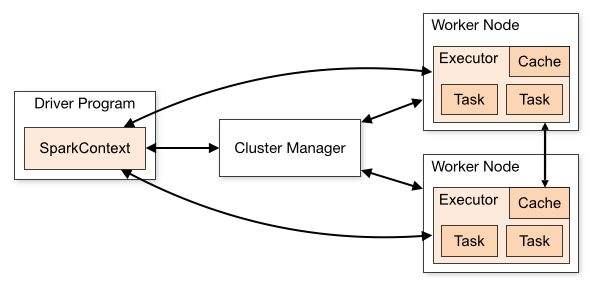
\includegraphics[scale=0.75]{Figures/spark_architecture.png}
	\decoRule
	\caption[Architettura Spark]{Architettura Master Slave}
	\label{fig:Architettura Spark}
\end{figure}

\subsection{Caratteristiche}
Spark si pone nel panorama del Data Processing come principale concorrente ad Hadoop MapReduce. Infatti, contrariamente alla controparte, fornisce l'opzione per lo Stream Processing e punta sull'analisi in tempo reale.\\
Per fare ciò l'architettura utilizza primitive "in-memory", lavorando direttamente in RAM laddove possibile. Questo approccio riduce di molto i tempi di latenza, rimuovendo l'overhead della scrittura su disco. Proprio per queste caratteristiche Spark viene preferito per algoritmi di apprendimento automatico e analisi dati interattiva, che richiedono accesso ripetuto agli stessi dati.

\subsection{Struttura}
Spark è organizzato su due livelli di librerie: uno fondamentale costituito da Spark Core e uno composto dalle estensioni incluse nativamente. Tra le principali in questa situazione riconosciamo:
\begin{itemize}
	\item \textbf{Spark SQL}, per l'interazione con dati strutturati
	\item \textbf{Spark Streaming}, orientata allo Stream Processing
	\item \textbf{MLlib}, che fornisce algoritmi di Machine Learning
	\item \textbf{GraphX}, adottata per il Graph Processing
\end{itemize}  

\begin{figure}[h]
	\centering
	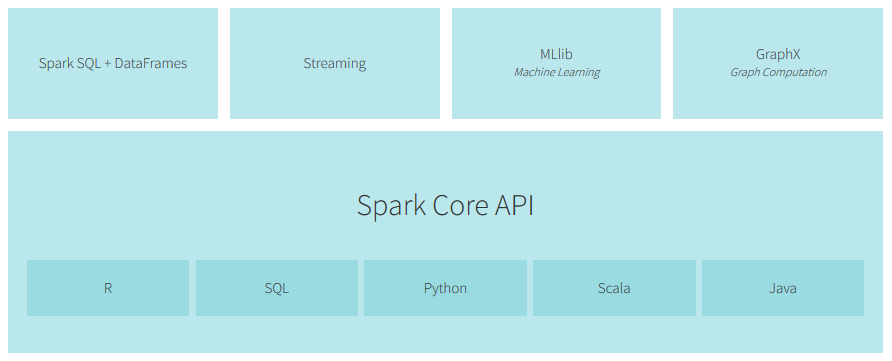
\includegraphics[scale=0.75]{Figures/spark_structure.png}
	\decoRule
	\caption[Struttura Spark]{Struttura Spark}
	\label{fig:Struttura Spark}
\end{figure}

\subsubsection{Spark Core}
Spark Core costituisce le fondamenta dell'intero framework, fornendo metodi di base relativi a scheduling e I/O. Tuttavia tra le componenti principali abbiamo il sopracitato oggetto \textit{SparkContext}, che comunica a Spark come interagire con la struttura del cluster.\\

\begin{code}
	\label{code:SparkContext}
	\begin{minted}[breaklines, breakbefore=., breakafter=(]{Scala}
    val conf = new SparkConf().setAppName(appName).setMaster("yarn")
    val spark = new SparkContext(conf) 
	\end{minted}
\end{code}~\\
È importante ricordare che ogni applicazione può avere solo un oggetto SparkContext attivo alla volta e, pertanto, bisogna ricorrere al metodo \textit{stop()}, qualora ci fosse la necessità di cambiarlo.

\paragraph{RDD} Gli RDDs (Resilient Distributed Datasets) \cite{spark_rdd_doc} sono collezioni di dati immutabili, tipate e distribuite che costituiscono la struttura dati caratteristica di Apache Spark, su cui si basano le ulteriori astrazioni che vengono applicate dalle librerie specifiche (Dataframes, Datasets).\\
Vengono generati a partire da riferimenti ad un sistema di memorizzazione esterno (es. HDFS) o "parallelizzando" una struttura dati già inizializzata nel programma. In questo modo il dato viene suddiviso in base alla struttura distribuita del cluster in partizioni logiche.\\
Supportano due tipi di operazioni: 

\begin{itemize}
	\item \textbf{Trasformazioni}: generano un nuovo RDD che andrà a prendere il posto di quello precedente. Questo perché i RDD sono immutabili in modo da garantire un sistema robusto ai potenziali problemi dovuti all'aggiornamento di risorse parallele. Sono definite "lazy", ossia il risultato non viene calcolato fino a quando non risulta necessario, in modo da evitare inutili sprechi di risorse e ottimizzare l'ordine delle operazioni laddove possibile. Ne sono esempi \textit{map}, \textit{filter} o \textit{join}.
	
	\item \textbf{Azioni} le operazioni che accedono al RDD per restituire un risultato tipato. Sono coloro che innescano l'esecuzione delle trasformazioni. Ne sono esempi \textit{reduce}, \textit{collect} e \textit{count}. 
\end{itemize}
Laddove possibile trasformazioni e azioni vengono effettuate direttamente in memoria, che viene liberata una volta che l'operazione è terminata. Questo garantisce prestazioni decisamente maggiori rispetto ai frameworks che lavorano "on-disk", rimuovendo i pesanti tempi di accesso necessari a interrogare il disco. Tuttavia talvolta può essere richiesto una persistenza del dato in memoria, in modo da rendere le future operazioni su quella risorsa più veloci; questo viene ottenuto tramite i metodi \textit{persist} e \textit{caching}, specificando il livello di memorizzazione necessario (es. MEMORY\_ONLY, DISK\_ONLY). Questa soluzione viene adoperata in particolare per algoritmi iterativi o interrogazioni rapide del dato, in quanto rende le future operazioni sulla risorsa fino a dieci volte più veloci.\\
I RDD godono infine di una politica di "fault tolerance" basata sul concetto di "lineage": viene mantenuta la cronologia delle operazioni  che hanno portato allo stato attuale sottoforma di DAG (Direct Acyclic Graph) e, in caso di errore del sistema, le partizioni vengono ricomputate per ripristinare lo stato corrente. Questo è possibile poiché il meccanismo di partizionamento è un processo deterministico, dunque riproducibile ripercorrendo la storia della risorsa. \newline

\subsection{Estensioni}

\subsubsection{GraphX}

GraphX \cite{spark_graph_doc} è un'estensione di Spark per grafi e analisi su di essi. Utilizza come astrazione di base l'oggetto "Property Graph" derivato dal RDD e mette a disposizione operatori proprietari e operatori ottimizzati derivati dalle API Pregel.

\paragraph{Property Graph}
L'entità Property Graph, o solo Graph, è un multigrafo, cioè un grafo con molteplici rami paralleli con vertici in comune, diretto con proprietà definite per ogni ramo e vertice, semplificando la descrizione di relazioni multiple tra coppie di nodi. GraphX riesce a ottimizzare le risorse per la memorizzazione del grafo relativamente al tipo di dato presente al suo interno, utilizzando tipologie diverse di array specializzati.\\
Derivano dai RDDs, i Property Graph condividono con essi tutte le caratteristiche di base già viste:
 
\begin{itemize}
	\item \textbf{Immutabili}: cambiamenti ai valori di un grafo implicano la creazione di uno nuovo che ne prenderà il posto. Per ottimizzare il processo vengono esclusi dalla ricomputazione tutti quei campi non interessati dalla trasformazione.
	
	\item \textbf{Distribuiti}: sono partizionati tra i processi di esecuzione utilizzando alcune tecniche di partizionamento di vertici.
	
	\item \textbf{Fault-tolerant}: mantengono lo stesso archetipo in materia, utilizzando il concetto di "lineage" per ricreare il grafo nel caso di errori di sistema.
\end{itemize}
Tale legame con il concetto di RDD si riflette nella struttura effettiva del Property Graph, che contiene come attributi due oggetti di tipo VertexRDD e EdgeRDD, versioni ottimizzate per vertici e rami della struttura dati.

\paragraph{Operatori}
In aggiunta all'oggetto Graph, il framework mette a disposizione una serie di operatori di base per applicare trasformazioni e azioni ai grafi. Questi sono riuniti sotto la classe \textit{GraphOps}, ma, se si sta utilizzando la versione in Scala del framework, sono disponibili direttamente come metodi del grafo tramite il meccanismo degli \textit{implicits}. Tra le principali famiglie riconosciamo:

\begin{itemize}
	\item \textbf{Operatori di proprietà}: equivalenti del \textit{map} del RDD, sono versioni specifiche e ottimizzate per operare su rami, vertici o le terne definite da "origine - ramo - destinazione", per considerare ogni istanza di una relazione.
	
	\item \textbf{Operatori strutturali}: operano sulla topologia strutturale del grafo, ad esempio \textit{reverse} o \textit{mask}.
	
	\item \textbf{Operatori di join}: consentono di estendere il grafo con dati provenienti da altri grafi o strutture dati esterne (es. RDD).
\end{itemize}

\subsubsection{Spark SQL}
Spark SQL \cite{spark_sql_doc} è il modulo dedicato all'analisi su dati strutturati e semi-strutturati, combinando le carateristiche di Spark con le ottimizzazioni di SQL in ambito relazionale.

\paragraph{DataFrame} Il DataFrame è l'astrazione che estende il RDD per rappresentare la struttura tabellare, tipica dell'ambiente SQL: è, infatti, fondamentalmente un RDD di righe con uno schema ben definito. Può essere generato da un RDD, deducendone lo schema o utilizzandone uno specificato esplicitamente, o a partire da un file da una sorgente esterna:

\begin{itemize}
	\item Json
	
	\item Csv
	
	\item Parquet
	
	\item JDBC
\end{itemize}

\subparagraph{DataFrame APIs}
I DataFrames implementano APIs sullo stile degli operatori SQL, trasposti nel paradigma introdotto dai RDD. Le \textbf{Trasformations} sono operazioni che danno in ritorno un altro oggetto di tipo DataFrame e sono "lazy", ossia non eseguiti se non quando viene richiesto un risultato tramite una Action. Ne sono alcuni esempi \textit{select()}, \textit{groupBy()} e \textit{join()}. Le \textbf{Actions} sono operazioni che restituiscono oggetti diversi da DataFrame e sono quelle che innescano l'effettiva esecuzione delle Transformations precedenti. Ne sono esempi \textit{count()}, \textit{collect()} e \textit{show()}.

\subparagraph{Ottimizzazione} 
Il connubio tra Spark e SQL permette di sfruttare il meglio di entrambi gli ambienti per generare ottimizzazioni sulle operazioni che riguardano i DataFrames. Queste possono avvenire però solo su dati appartenenti ad una ristretta cerchia:

\begin{itemize}
	\item Tipi di dato numerici
	\item Timestamp e Date
	\item String
	\item Array e Map
	\item Case Class
\end{itemize}
Le ottimizzazioni avvengono tramite due componenti del backend di Spark SQL.\\
\textbf{Catalyst} si occupa dell'ottimizzazione per le query effettuate sui DataFrames. Questo perché la struttura fornisce una gran quantità di metadati rispetto al RDD su cui lavorare. La maggior parte dei miglioramenti vengono effettuati riordinando le operazioni richieste, grazie alla "laziness" delle Trasformations, e effettuando per ogni operazione solo la lettura dei dati necessari.\\
\textbf{Tungsten} offre un servizio di encoding dei dati "off-heap" che, grazie alle limitazioni relative ai tipi di dati utilizzabili, può gestire al meglio quelli permessi. 

\begin{itemize}
	\item Gestisce la serializzazione del dato in memoria, minimizzando lo spazio occupato e velocizzando il processo di serializzazione e deserializzazione.
	\item Riconosce quali operazioni lavorano per righe e quali per colonne, cambiando contesto a seconda della necessità.
	\item Opera "off-heap", in modo da evitare i rallentamenti dovuti alla garbage collection.
\end{itemize}

\paragraph{SQL Literals} Uno dei principali concetti che mette a disposizione Spark SQL è quello dei SQL Literals, che permettono di applicare queries in stile SQL direttamente sui DataFrame, garantendo un legame con le tecnologie precedenti e venendo incontro a chi è abituato al diffuso linguaggio di query. Tutti i principali operatori sono supportati:

\begin{itemize}
	\item SELECT, FROM, WHERE
	\item DISTINCT, HAVING
	\item GROUP BY, ORDER BY
	\item Operatori JOIN
	\item Subqueries
\end{itemize}

\subsubsection{Spark Streaming}
Spark Streaming \cite{spark_stream_doc} è l'estensione che si occupa di elaborazione di dati in tempo reale, sfruttando tutte le potenzialità offerte dall'ambiente Spark. In questo modo le APIs forniscono uno strumento scalabile e "fault-tolerant" per analizzare i dati provenienti da un flusso di dati, garantendo un elevato flusso di produzione. Supporta le principali fonti di "ingestion streams", quali Kafka o NiFi e sorgenti esterne come Amazon Kinesis o filesystems (HDFS, S3).\\
Il dato viene assimilato e organizzato in mini-batches, su cui possono essere effettuate le operazioni tipiche del "Batch Processing", utilizzando funzioni di alto livello quali map, reduce e join. Il risultato può essere poi inoltrato ad un filesystem, un database distribuito o nuovamente come stream di dati.

\begin{figure}[h]
	\centering
	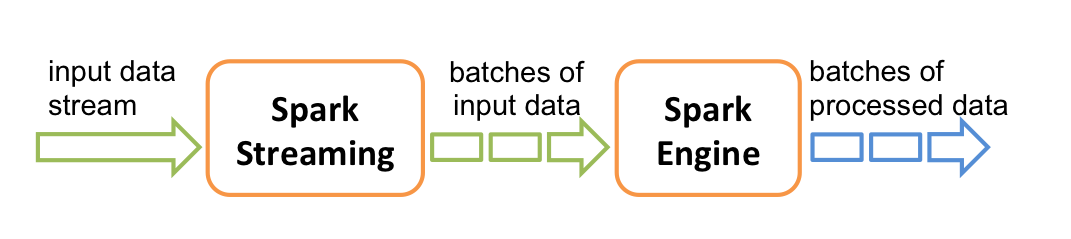
\includegraphics[scale=0.75]{Figures/spark_streaming.png}
	\decoRule
	\caption[Struttura Spark Streaming]{Struttura Spark Streaming}
	\label{fig:Struttura Spark Streaming}
\end{figure}

\paragraph{DStream}
DStream (Discretized Stream) è la principale astrazione utilizzata dalla libreria, che rappresenta uno stream di dati continuo. Può essere generato da una sorgente esterna tra quelle menzionate precedentemente o applicando una trasformazione ad un altro DStream.\\
Le somiglianze con il RDD derivano dal fatto che internamente l'oggetto viene considerato come una sequenza di RDDs, uno per ciascun mini-batch in cui viene discretizzato il flusso di dati in input, mantenendo le caratteristiche di fault-tolerance e parallelismo tipiche della struttura dati che estende.\\
Una volta ottenute le mini-batches, queste passano all'elaborazione con i metodi di Spark, generando corrispondenti batches di dati processati. Questo chiaramente introduce una minima latenza, dovuta alla dimensione del segmento in cui viene suddiviso il flusso di dati.

\subsubsection{MLlib}
La libreria MLLib \cite{spark_mllib_doc} o Machine Learning Library è un estensione di APIs per Spark che fornisce molteplici strumenti e algoritmi per il Machine Learning, con l'obbiettivo di rendere tale approccio semplice e scalabile su grandi moli di dati, sfruttando il paradigma "in-memory" fornito da Apache Spark.\\
Sono disponibili due tipi di APIs, una basata su DataFrame e l'altra su RDD, con quest'ultima che verrà lentamente abbandonata in favore della maggiore semplicità d'uso offerta dal DataFrame.

\paragraph{Gli strumenti} 
MLLib mette a disposizione una pletora di classi e metodi da affiancare agli algoritmi di analisi. Si tratta di classi che spaziano dalla manipolazione e pulizia del dato per adattarlo alla forma richiesta all'ottimizzazione degli iperparametri del modello scelto.

\subparagraph{ML Pipeline} 
Permette di definire le fasi dell'analisi che vogliamo effettuare, raccogliendo i vari passaggi in un'unica sequenza, i \textit{PipelineStages}. In questo modo siamo certi che tutte le operazioni vengano effettuate sul dato, riducendo lo spazio ad errori di sorta.\\
I passaggi possono essere \textit{Transformers}, che trasformano il Dataframe in un altro (es. modificando o aggiungendo colonne), o \textit{Estimators}, astrazione che racchiude tutti gli algoritmi di apprendimento. Mentre gli oggetti \textit{Transformers} implementano solo il metodo \textit{transform()}, usato per applicare l'operazione specificata al dato, gli oggetti di tipo \textit{Estimators} hanno anche un metodo \textit{fit()}, necessario a effettuare il training sui dati specificati e generare il corrispondente modello e diventando un \textit{Transformer}.\\ 
La Pipeline stessa è un \textit{Estimator} e necessita, dunque, di entrambe le operazioni. Una volta definiti gli stages viene chiamato il metodo \textit{fit()}, che viene applicato secondo l'ordine specificato a tutti gli \textit{Estimators} presenti tra gli stages. Viene così generato un \textit{PipelineModel} (o \textit{Fitted Pipeline}), che a questo punto rappresenta una raccolta di soli oggetti \textit{Transformers}. Infine il metodo \textit{transform()} viene applicato su ogni stage sequenzialmente, applicando il modello complessivo al dato considerato.

\subparagraph{ML Tuning} 
Suite di oggetti dedicata all'ottimizzazione dei parametri dei modelli, nota anche come \textit{model selection}. Ne fanno parte:
\begin{itemize}
	\item \textbf{CrossValidator}: classe che applica la tecnica della Cross Validation, congiunta con un ottimizzazione dei parametri specificati del modello. Il dataset viene suddiviso in più partizioni, chiamate \textit{folds}, ognuna delle quali viene alternatamente considerata come testing set e le rimanenti come training set.
	\item \textbf{TrainValidationSplit}: contrariamente alla precedente si concentra solo sull'ottimizzazione dei parametri, effettuando solo una volta la divisione del dataset secondo la frazione specificata.
\end{itemize}
Ciascuno di questi strumenti necessita di tre elementi: 
\begin{itemize}
	\item \textbf{Estimator}: algoritmo o \textit{Pipeline}, soggetto dell'ottimizzazione.
	\item \textbf{ParamMaps}: parametri e relativi intervalli di valori tra cui vogliamo scegliere il modello migliore.
	\item \textbf{Evaluator}: oggetto che fornisce il criterio discriminante nella valutazione. 
\end{itemize}
Il procedimento dunque prevede la suddivisione del dataset secondo la logica specifica. Per ciascuna coppia di training set e testing set ottenuta in questo modo si itera tra i valori specificati dalle \textit{ParamMaps} e viene selezionato il modello migliore, che viene mantenuto come attributo \textit{bestModel} della classe.

\subparagraph{Feature Transformers} 
Oltre a strumenti più prettamente legati all'aspetto pratico dell'analisi del dato, MLlib mette a disposizione oggetti che si occupano di supportare lo sviluppatore nel modificare la forma delle strutture dati in suo possesso in modo da renderle conformi all'algoritmo o modello selezionato.
\begin{itemize}
	\item \textbf{Tokenizer}: suddivide un testo unico nelle singole parole di cui è composto. Nel caso si volesse avere maggiore controllo sul processo di segmentazione si può ricorrere a \textit{RegexTokenizer}, che permette di specificare la regola da utilizzare tramite espressione regolare (regex).
	\item \textbf{Indexers}: permettono di convertire dati non numerici in numerici, per inserirli come input in modelli o altri operatori. A seconda del tipo di dato che ci troviamo a trattare si ricorre a \textit{StringIndexer}, per input testuali, o a \textit{VectorIndexer}, nel caso di un Vector. In entrambi i casi il dato risultato è una codifica univoca in Double, basata sulla frequenza della singola istanza.
	\item \textbf{Bucketizer}: applicato su una colonna a valori continui, genera segmenti di dominio secondo la logica specificata e applica a ogni elemento il valore della partizione corrispondente, discretizzando la misura.
	\item \textbf{VectorAssembler}: genera un'unica colonna di tipo Vector a partire da molteplici colonne. Viene utilizzato per preparare l'input ad alcuni modelli che richiedono una colonna per rappresentare le feature su cui eseguire l'algoritmo.
\end{itemize}

\paragraph{Gli algoritmi}
Una delle caratteristiche più apprezzate di MLlib risiede nella grande quantità di algoritmi di Machine Learning implementati nativamente:
\begin{itemize}
	\item \textbf{Classificazione}: Linear SVM, Naive Bayes
	\item \textbf{Regressione}: Regressione Lineare, GLM
	\item \textbf{Clustering}: K-Means
	\item \textbf{Tree} e \textbf{Ensembles}: Decision Tree, Random Forest, GBT
\end{itemize}
\pagebreak


\chapter{Le Misure di Sicurezza}

Dal momento che i dati che trattiamo e ricaviamo dall'analisi hanno rilevanza conoscitiva e valore in termini di mercato e ricerca, risulta fondamentale considerare un ambiente sicuro in cui accogliere tali informazioni. Il perimetro deve però garantire, contemporaneamente alla discrezione relativamente all'accesso del dato, un livello sufficiente di astrazione per le interazioni esterne.\\
La struttura progettata risulta articolata su due livelli:
\begin{itemize}
	\item \textbf{Frontend}: si occupa dell'interazione dell'utente con i servizi forniti dal cluster;
	\item \textbf{Cluster}: i nodi sottostanti, che garantiscono un livello di sicurezza più specifico per ogni servizio interpellato.
\end{itemize}
Il primo problema da porsi nello sviluppo di una struttura di sicurezza risulta essere la definizione delle entità che possono interagire con il sistema e in quale misura tali interazioni avvengono, in modo da fornire una soluzione adatta sia in termini di confidenzialità per le parti che per facilità d'uso.\\
Parliamo, quindi, di:
\begin{itemize}
	\item operatori tecnici: sviluppatori o amministratori del sistema, che necessitano di accessi più profondi e possono lavorare all'interno della rete aziendale.
	\item utenti esterni: clienti o personale generico, che necessitano di utilizzare i servizi del cluster, senza possibilità di modificarne la struttura.
	\item sorgenti dati: data streams esterni, inviano dati su cui si lavorerà con gli strumenti presenti nel cluster.
\end{itemize}
Per ciascun utente si considerano approcci differenti, commisurati alle esigenze. Le richieste avvengono su un ristretto numero di porte abilitate alla comunicazione con l'esterno e viaggiano su canali sicuri, tramite l'utilizzo di protocolli quali HTTPS, SSH e FTPS.\\
In un secondo momento le chiamate vengono autenticate tramite provider dedicati come LDAP o Kerberos, per poi essere sottoposte ad un controllo di autorizzazione, atto a verificare che la richiesta sia congrua ai diritti dell'utente.\\
L'esito di ciascun passaggio viene registrato da un servizio di auditing, che permette di tenere traccia delle richieste e degli accessi al sistema, in modo da identificare eventuali abusi o tentativi di forzatura del sistema.\\
\begin{figure}[h]
	\centering
	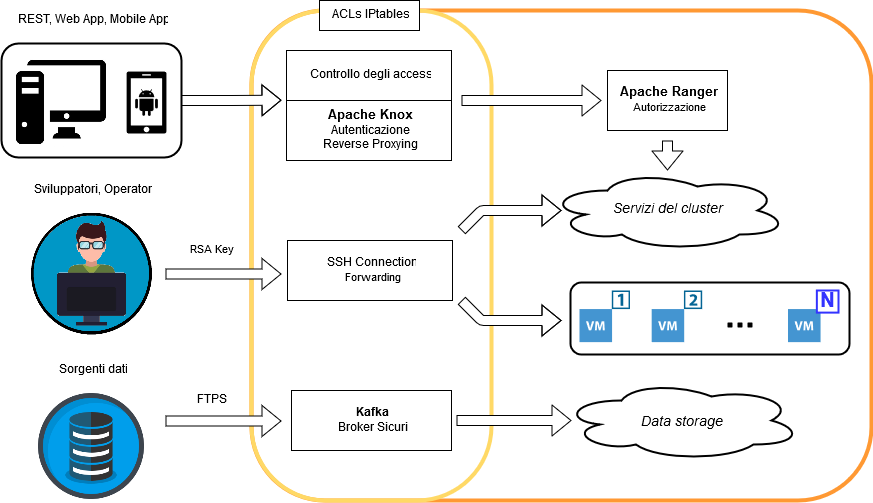
\includegraphics[scale=0.4]{Figures/security_diagram.png}
	\decoRule
	\caption[Struttura Sicurezza]{Struttura del perimetro di sicurezza}
	\label{fig:security_diagram}
\end{figure}
\pagebreak

\section{Knox}

Apache Knox \cite{knox_doc} è un Application Gateway, componente della suite di strumenti Hadoop, che fornisce varie funzionalità in termini di sicurezza per clusters Hadoop, specialmente se coadiuvato da altri elementi.
\newline
Nella struttura in esame riveste il ruolo fondamentale di "Reverse Proxying" dei servizi offerti dal cluster e di autenticazione e "Access Control".

\subsection{Reverse Proxying}
Il gateway Knox fornisce un servizio di mascheramento che permette di definire un URL da mostrare all'utente esterno corrispondente a ciascuna chiamata rivolta al cluster. In questo modo è possibile distinguere interfaccia e implementazione del servizio, mantenendo confidenziale la struttura dell'architettura sottostante e garantendo la modularità del sistema.\\
Ogni servizio che necessiti di Knox deve essere dichiarato all'interno di uno specifico file di topologia. La topologia è un file XML che dichiara le componenti associate a Knox, quali provider di autenticazione e autorizzazione, e i servizi gestiti dal file in esame.
A questo vengono accompagnati due file di definizione del servizio:
\begin{itemize}
	\item \textbf{service.xml}: definisce la struttura della chiamata che verrà associata al servizio interessato.
	\item \textbf{rewrite.xml}: definisce tramite regex la politica di riscrittura che deve essere seguita, prima che la chiamata venga inoltrata al cluster.
\end{itemize}
Le chiamate che possono essere fatte tramite Knox seguono i dettami del protocollo REST, riportando indirizzo, topologia e servizio richiesto nell'URL sottoposto.

\subsubsection{Funzionamento}
Nel momento in cui una richiesta arriva al sistema comincia il processo che porta alla conversione dell'URL pubblico in quello riconosciuto dai nodi interni al cluster.
\begin{itemize}
	\item Dall'URL viene ricavata la topologia da utilizzare, in modo da fare riferimento ai provider e alle definizioni dei servizi corrispondenti.
	\item L'URL viene riconosciuta come appartenente a un particolare servizio, dichiarato all'interno della topologia selezionata.
	\item Secondo il contenuto dei relativi file "service.xml" e "rewrite.xml" la stringa viene convertita nella forma non mascherata e inoltrata al servizio di dovere all'interno del cluster. 
\end{itemize}

\subsection{Autenticazione e Access Control}
Il gateway Knox si presenta come unico access point sicuro per le interazioni con il cluster, che siano esse tramite API REST che attraverso chiamate HTTP/HTTPS. Ogni richiesta viene inoltrata previa sottomissione di credenziali. Queste vengono autenticate da Knox tramite il provider dichiarato dalla topologia selezionata, LDAP o Kerberos.
Successivamente la chiamata autenticata viene sottoposta all'entità specificata per l'autorizzazione che garantisce controllo sugli accessi ai servizi del sistema.
Infine, una volta garantita la bontà della richiesta, viene sottoposta al servizio per l'esecuzione.

\pagebreak

\section{Ranger}

Apache Ranger \cite{ranger_doc} è un framework che si occupa di definire e gestire la sicurezza del dato all'interno di un cluster Hadoop. Questo avviene tramite l'utilizzo di un sistema di autorizzazione specifico per ogni servizio presente nel cluster che centralizza le logiche di autorizzazione per le varie risorse del sistema. La gestione di Ranger può avvenire sia tramite interfaccia grafica web, sia tramite chiamate REST al nodo su cui risiede il framework. Infine, garantisce una profonda conoscenza per quanto riguarda le interazioni con il cluster, tramite un servizio di audit che osserva le operazioni effettuate in tempo reale e le registra su HDFS o Solr.

\subsection{Autorizzazione}

Nel momento in cui una richiesta a un servizio del cluster viene autenticata dal provider scelto, deve essere sottoposta al controllo di Ranger, per verificare i privilegi dell'utente nei confronti della risorsa richiesta. È possibile gestire il processo di autorizzazione su due livelli differenti: discriminando rispetto caratteristiche di chi effettua l'accesso o a che unità di lavoro appartiene (access authorization) o relativamente alla risorsa richiesta (resource authorization).
\newline 
All'interno di tali approcci possiamo riconoscere ulteriori distinzioni. Relativamente al controllo degli accessi degli utenti:
\begin{itemize}
	\item Role based \textbf{RBAC}: valuta l'accesso in base a criteri di ruolo e privilegi dell'utente.
	\item Attribute based \textbf{ABAC}: una specializzazione del RBAC, che considera nella valutazione anche attributi aggiuntivi, come indirizzo IP, luogo di login o dati dell'utente.
\end{itemize}
Per quanto riguarda,invece, l'accesso alle risorse, essendo un framework rivolto all'utilizzo in un ambiente Hadoop, Ranger mette a disposizione alcuni plugin per interagire direttamente con i principali servizi presenti nella suite, garantendo un controllo più specifico e profondo riguardo quali operazioni l'utente possa e non possa fare. I plugin sono programmi in Java incapsulati in processi del servizio di riferimento che si occupano di caricare le regole da un server centrale e memorizzarle localmente in un file. Tra i servizi riconosciuti troviamo:
\begin{itemize}
	\item HDFS
	\item HBase
	\item Hive
	\item Yarn
\end{itemize}
Ad esempio, per quanto riguarda Hive, le regole di autorizzazione permettono di specificare per ogni regola quali operatori è possibile utilizzare nelle query al database, chi può effettuarle e a quali campi può avere accesso.

\subsection{Regole "Tag Based" e persistenza dei dati}

Versioni più recenti di Ranger hanno introdotto la possibilità di utilizzare regole di sicurezza basate su etichette. Queste vengono attribuite a varie risorse dai vari servizi in modo da definire lo stesso tipo di regola per entità differenti senza doverlo definire esplicitamente, rendendo più semplice le operazioni di controllo degli accessi e di gestione delle risorse. Le etichette e la loro definizione sono tenute in un "Tag Store", mentre un processo di sincronizzazione TagSync si occupa di mantenere le informazioni sempre aggiornate tra i servizi che ne fanno uso.
\newline
Tutte i dati relativi alla logica di sicurezza sono memorizzati in locale, in uno database MySQL su uno degli hosts, che mantiene tutte le informazioni relative a regole e utenti previsti dal framework. La coerenza del sistema viene garntita da un processo di sincronizzazione dedicato che aggiorna le liste di utenti, gruppi e ruoli con LDAP/Active Directory e le opzioni di configurazione con Ambari.
\chapter{Prevedere i Ritardi Aerei: un caso d'uso}

\section{Introduzione}

\pagebreak

\section{L'Infrastruttura}

\subsection{Hardware}

\pagebreak

\subsection{Data Management \& Access}
\subsubsection{HDFS}
Hadoop Distributed File System (\textbf{HDFS}) \cite{hadoop_doc} è uno dei principali file system distribuiti del settore, grazie alla sua scalabilità con cui garantisce elevate prestazioni e facilità di utilizzo anche su clusters di grandi dimensioni.

\paragraph{Architettura}
HDFS segue la struttura \textbf{master-slave}, con due livelli di componenti che interagiscono tra loro:
\begin{itemize}
	\item \textbf{NameNode}: ricopre il ruolo del \textit{master}, occupandosi della gestione del namespace del filesystem e del controllo degli accessi ai dati da parte dei vari clients. Espone un'interfaccia organizzata secondo la classica gerarchia a cartelle, mantenendo metadati riguardo al contenuto e la struttura, e si occupa di organizzare la distribuzione dei blocchi di dato nei vari DataNodes.
	
	\item \textbf{DataNodes}: sono gli \textit{slaves}, che effettuano le operazioni di lettura e scrittura insieme a operazioni di base sui blocchi di dato, tutte ordinate dal NameNode. 
\end{itemize}

\paragraph{Fault Tolerance}

L'utilizzo di un cluster composto da più dispositivi comporta un aumento consistente nel rischio di perdita dei dati: un qualunque guasto può avere ripercussioni su altre componenti che dipendono da esso. Per questo è ancora più rilevante avere una politica affidabile di reazione a tali inconvenienti.\\
HDFS gestisce questa eventualità in prima istanza prevenendo situazioni critiche: quando un file viene salvato il NameNode non ordina una sola scrittura di esso, ma più blocchi vengono scritti su molteplici DataNodes, relativamente al corrispondente parametro di ridondanza \textbf{Replication Factor}. In questo modo il dato risulta sempre disponibile anche nella sfortunata evenienza di un malfunzionamento.\\
Questo criterio, in congiunzione con i metadati salvati per ogni operazione, permette di ripristinare la situazione anche nel caso di errore dello stesso HDFS. Ogni modifica e lo stato attuale del filesystem sono costantemente mantenuti rispettivamente nel \textbf{EditLog} e \textbf{FsImage}, entità che vengono adoperate al riavvio del NameNode per effettuare nuovamente le recenti operazioni.

\subsubsection{YARN} 
Yet Another Resource Negotiator \cite{yarn_doc} (\textbf{YARN}) è il sistema operativo distribuito della suite Hadoop. Riveste il ruolo di gestore delle applicazioni distribuite che vengono eseguite sul cluster: si occupa dell'affidamento delle risorse e dello scheduling dei jobs.

\paragraph{Architettura}
La struttura di YARN è articolata su due \textit{daemons}:
\begin{itemize}
	\item \textbf{Resource Manager}: supportato dai \textbf{Node Managers}, rappresenta il framework di elaborazione sui dati e scheduler. Si occupa di distribuire le risorse per i vari jobs ai nodi, dove il controllo passa al singolo Node Manager della macchina. Questo di assicura di attribuire a ciascuna applicazione il proprio \textit{container}, in modo da isolarne l'ambiente di esecuzione, e fare rapporto al Resource Manager dell'utilizzo delle risorse del nodo.
	
	\item \textbf{Application Master}: si occupa della richiesta di risorse per la singola applicazione cui è legato al Resource Manager. Quando viene lanciato un'applicazione, che consiste in un job o in un DAG di job, il relativo Application Master ottiene un container per l'esecuzione iniziale. Da questo momento l'AM interagisce con il relativo Node Manager, condividendo con esso le informazioni di avanzamento del processo e lo stato del container.
\end{itemize}

\subsubsection{Hive}

\pagebreak

\subsection{Data Ingestion}

\subsubsection{Kafka}

\pagebreak

\subsection{Data Visualisation}

\subsubsection{Tableau}

\pagebreak

\subsection{Servizi Accessori}

\subsubsection{REST APIs}

\paragraph{Arnia}

\paragraph{KhanUI}

\subsubsection{Push Notification}

\paragraph{NotiFire}

\pagebreak

\section{Dal Dato alla Previsione}

\subsection{Apprendimento}

\pagebreak

\subsection{Previsione}

\pagebreak

\subsection{Analisi dei Risultati}

\pagebreak

\section{Sicurezza}

\chapter{Conclusioni}

%----------------------------------------------------------------------------------------
%	THESIS CONTENT - APPENDICES
%----------------------------------------------------------------------------------------

%\appendix % Cue to tell LaTeX that the following "chapters" are Appendices

% Include the appendices of the thesis as separate files from the Appendices folder
% Uncomment the lines as you write the Appendices

%% Appendix A

\chapter{Frequently Asked Questions} % Main appendix title

\label{AppendixA} % For referencing this appendix elsewhere, use \ref{AppendixA}

\section{How do I change the colors of links?}

The color of links can be changed to your liking using:

{\small\verb!\hypersetup{urlcolor=red}!}, or

{\small\verb!\hypersetup{citecolor=green}!}, or

{\small\verb!\hypersetup{allcolor=blue}!}.

\noindent If you want to completely hide the links, you can use:

{\small\verb!\hypersetup{allcolors=.}!}, or even better: 

{\small\verb!\hypersetup{hidelinks}!}.

\noindent If you want to have obvious links in the PDF but not the printed text, use:

{\small\verb!\hypersetup{colorlinks=false}!}.

%\include{Appendices/AppendixB}
%\include{Appendices/AppendixC}

%----------------------------------------------------------------------------------------
%	BIBLIOGRAPHY
%----------------------------------------------------------------------------------------

\printbibliography[heading=bibintoc]

%----------------------------------------------------------------------------------------

\end{document}  
